\section{Background}

\subsection{Why use Bluetooth Low Energy (BLE) for proximity detection}

Experiments have been performed indicating that RSSI is a viable mean for proximity detection \cite{ref:Takashi}. 

It is important that the proximity detection is implemented without pairing any devices. This is to make the authentication as seamless as possbile, by saving the user from spending time pairing the devices manually.

BLE has been chosen for this project for the following reasons:
\begin{itemize}
	\item BLE has low power consumption when set to use the BLE periphal role. The periphal role is enough for the phone devie and in a real life scenario the Bluetooth might need to be turned on for sevreal hours.
	\item BLE allows a small amount of communication without pairing devices, which allows the system to discover and receive addresses of the devices in the immediate vicinity. This enables the system to determine if a given device is registered to a user of the system without pairing with the device.
\end{itemize}

BLE is a fairly new standard and as such not all devices supports it yet. However this is outweighed by the what is gained from choosing BLE. 

Currently BLE is amongst other supported by a number of cell phones and wearables see \cref{table:devices}.

\begin{table}[!t]
\caption{Device descriptions}
\label{table:devices}
\centering
% Some packages, such as MDW tools, offer better commands for making tables
% than the plain LaTeX2e tabular which is used here.
\begin{tabular}{|p{2.3cm}|p{1.3cm}|p{3.9cm}|}
\hline
\textbf{Device} & \textbf{Hardware Support} & \textbf{Software Support}\\
\hline
iPhone 5, iPhone 5s (IOS7) & Yes & Yes\\
\hline
Nexus 5 \newline (Kitkat 4.4.2) & Yes & Partial \newline
Central role (Android 4.3)  \newline
peripheral role (Android~L)\\
\hline
Pebble Smartwatch (Pebble OS 2.0) & Yes & Peripheral role\\
\hline
\end{tabular}
\end{table}

\subsection{Security}

Authenticating a user when the user is close to the system introduces some security issues, which needs to be addressed differently depending on the system. One could imagine a partial login authentication model where the user is only granted access to functionality, which does not need high level security, when the user is close and more functionality on top of what has already been given, when the user swipes a nfc card. 

In this case the user would only be granted access to lower level functionality, such as 'view-only', when being close the system. This would limit the rights of nearby authentication to reduce the impact it would have, should the nearby authentication be comprimised. 

%\subsection{Partial authentication model}
%A login method has been developed to take different levels of trust into account.
%As presented in \cref{fig_authentication_model} the authentication model has three levels of trust
%\begin{itemize}
%\item High (green)
%\item Medium (yellow)
%\item Low (red)
%\end{itemize}
%
%\begin{figure}[!t]
%	\centering
%	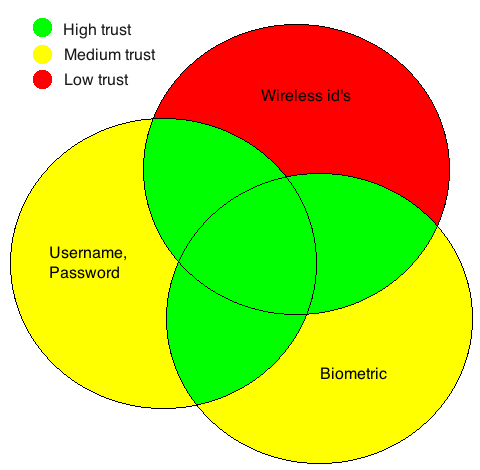
\includegraphics[width=2.5in]{img/authenticationModel}
%	\caption{ Partial login and trust }
%	\label{fig_authentication_model}
%\end{figure}
%
%High trust is obtained by authenticating with a combination of two of the three authentication methods.
%As shown in \cref{table_data_access} a user is only able to view and edit sensitive data within the high trust area of the model.
%
%Medium trust is obtained by authenticating with either a username/password or biometric authentication.
%These two authentication methods is reasonable secure and are used universally for authentication.
%A user that has obtained medium trust is able to view sensitive data but cannot edit or delete it.
%With medium trust a user can view and edit non sensitive data.
%
%Low trust is obtained by calm authentication with a Bluetooth enabled device.
%A user with low trust can view personal non sensitive data like a name or a personal todo-list.
%No edit or delete is allowed.
%
%This model allows the user to be partially authenticated before any physical interaction.
%The system gets the ability to recognize users and may for instance use that information to move a session started on one system to the current system so the user is able to seamlessly work on from the point the previous session ended.
%
%\begin{table}[!t]
%\caption{Data access}
%\label{table_data_access}
%\centering
%% Some packages, such as MDW tools, offer better commands for making tables
%% than the plain LaTeX2e tabular which is used here.
%\begin{tabular}{|p{1.3cm}|p{2.0cm}|p{2.0cm}|p{2.0cm}|}
%\hline
%\textbf{Trust} & \textbf{Non sensitive personal data} & \textbf{Non sensitive data} & \textbf{Sensitive data}\\
%\hline
%\textbf{High} & Read/Write & Read/Write & Read/Write\\
%\hline
%\textbf{Medium} & Read/Write & Read/Write & Read\\
%\hline
%\textbf{Low} & Read & - & -\\
%\hline
%\end{tabular}
%\end{table}
%
